%
%    18afmc template paper adapted from 14afmc template.
%
%    Format: LaTeX2e.
%
\documentclass[twocolumn]{afmc_art}
\usepackage{graphicx}
%
%
\begin{document}

%
%%%  Fill in following information.
%
%%%%%%%%%%%%%%%%%%%%%%%%%%%%%%%%%%%%%%%%%%%%%%%%%%%%%%%%%%%%%%%%%%%%%%%%%%%%
%
%    Contact Author: put your name here
%            E-mail: put your email address here
%             Phone: put your phone number here
%               Fax: put your fax number here
%
%%%%%%%%%%%%%%%%%%%%%%%%%%%%%%%%%%%%%%%%%%%%%%%%%%%%%%%%%%%%%%%%%%%%%%%%%%%%
%
%%%  Put your definitions (if any) here
%
%
%%%  Title goes here - do not force a line-break unless ABSOLUTELY necessary
%
\title{18th Australasian Fluid Mechanics Conference:\\
       Instructions to Authors Sample Paper}
%
%%%  Authors and affiliations with brief address 
%
%    format: 
%
\author{J.~P. Denier$^1$, P.~V. Lanspeary$^2$ and S.~E. Norris$^3$}
\affiliation{$^1$Department of Applied Mathematics\\
                Adelaide University, South Australia 5005, Australia\\[5pt]
             $^2$Department of Mechanical Engineering\\
             University of Adelaide, Adelaide, South Australia 5005, Australia\\[5pt]
             $^3$Department of Mechanical Engineering\\
             University of Auckland, Auckland 1142, New Zealand}

%
\maketitle
%
%%%  Paper proper starts here
%
\section{Abstract}
Include a brief abstract here.

\section{Introduction}
The conference proceedings will be published from
``camera-ready copy''. For reasons of uniformity, all papers must 
adhere to the format as defined by the appropriate document template,
the \texttt{afmc\_art} class file together 
with this ``template'' paper. 

The organising committee will accept papers formatted using either
the \LaTeX\ or Microsoft Word templates available on the web at\\
\centerline{\texttt{http://www.18afmc.com.au}}

Particular attention should be given to the 
formatting style used in this ``template''. 
Papers which do not conform to this style will
{\bf NOT} be published. 

For authors who use \LaTeX\ to prepare a paper,
this file serves as an ``instructions to authors'' and,
together with the \LaTeX\ class file \texttt{afmc\_art.cls},
it is the document template for 18AFMC papers.
\LaTeX\ users may begin by editing this file.
Note that anything after a \texttt{\%} is a comment and
is ignored by \LaTeX.
Lines beginning with \texttt{\%\%\%} require you to take some
action such as fill in the title.

\section{Submitting papers}

Please upload a PDF file of your paper for review to the 18AFMC web site
http://www.18afmc.com.au
by the due date, 17$^{\mbox{th}}$ August 2012.

\section{Page limits}
The page limit for contributed papers is four (4) pages. The page limit for 
invited papers is eight (8) pages. Papers which exceed this limit will be 
returned to the author(s) for shortening. 

\section{Title and Authors}
The title should be in lower case with the first letter of major words
capitalised. Avoid forcing a line-break unless absolutely necessary.
Author affiliations should consist of ``Department, Institution, City,
State, Post-code, Country''. Author affiliations should be indicated
with a superscript digit. 

\section{Section Headings}

\subsection{And Subsection Headings}

Section and subsection headings should be in lower case with the first 
letter of major words in upper case. Do not use subsubsections.

\section{Figures and Tables}

All figures should either be produced using the \LaTeX\ picture environment
or be saved as a postscript file and inserted in the text using the {\tt epsf}
macros. Figures and Tables should appear in the text near to where they are
first referenced. They should be centred between the margins, and must not fall
outside of the normal printed area of the page which is 170mm wide by 248mm 
high. The font size for all numbers and letters in the figure, as it appears
in your paper, must be at least as large as that for the running headings.
Put table captions below the table, and figure captions below the figure.
Refer to figures and tables as in ``figure 1, table 1''.

The proceedings will be distributed on a USB memory stick so colour figures and 
illustrations can be included. However, please try, where possible, to ensure 
that the details are still clear in black and white copies.

There are two possible \LaTeX\ environments for placing figures and
tables within the text. If you wish to have a table or figure that
spans both columns of the paper then you must use the environments 
\begin{verbatim}
\begin{table*}
\end{table*}
\end{verbatim}
and 
\begin{verbatim}
\begin{figure*}
\end{figure*}
\end{verbatim}
in order for the two column format to correctly
position tables and figures across the page.

If you wish to place a smaller table or figure (ie one which is less
than the column width of 80mm) then you should use the usual \LaTeX\
environments
\begin{verbatim}
\begin{table}
\end{table}
\end{verbatim}
and 
\begin{verbatim}
\begin{figure}
\end{figure}
\end{verbatim}
If you use a mixture of standard and $*$-forms
you will need to take some care to ensure that the 
double-column tables (or figures) do not appear out
of sequence.  If this occurs try placing the double
column table (or figure) at a later place in the text.

Some care should be taken when reducing the size of figures; make sure
that the figure and all labels are still legible.

\begin{table}[ht]
\centering
\begin{tabular}{|r|r|r|}
\hline
\multicolumn{3}{|c|}{Problem A}\\
\hline \hline
$40\times 40$&$80\times 80$&$160\times 160$\\ \hline
 129    & 258      &  520     \\
 0.179  & 1.844    & 8.527  \\
 2.8E-6 &  4.56E-6 & 4.5E-6  \\ \hline
\end{tabular}
\caption{This is an example of a table. Note that it is centred.}
\end{table}   

\begin{figure}[b]
\vspace{2mm}
\centering
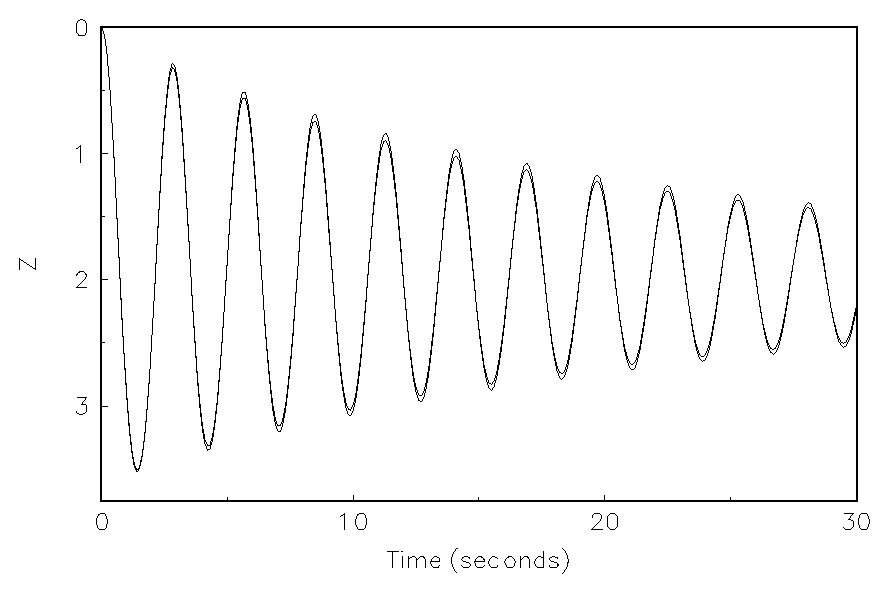
\includegraphics[width=0.4\textwidth]{fig.eps}
\caption{This figure was saved as an encapsulated Postscript file. It is also centred between the 
margins. Because the bounding box of this figure is fairly tight some
space has been added above the figure. This is not a good example
of a figure; the lines should be thicker and a bigger and bolder font
used.}
\end{figure}

\begin{table*}[ht]
\centering
\begin{tabular}{|r|r|r||r|r|r|}
\hline
\multicolumn{3}{|c||}{Problem A}&\multicolumn{3}{|c|}{Problem B}\\
\hline \hline
$40\times 40$&$80\times 80$&$160\times 160$&
$40\times 20$&$80\times 40$&$160\times 80$\\ \hline
 129    & 258      &  520   &   102   &   193   &  387     \\
 0.179  & 1.844    & 8.527  &   0.148 &   0.700 &  4.468   \\
 2.8E-6 &  4.56E-6 & 4.5E-6 &  3.1E-6 &  3.2E-6 &  4.2E-6  \\ \hline
\end{tabular}
\caption{This is an example of a table. Note that it is centred.}
\end{table*}   

\begin{figure*}[ht]
\centering
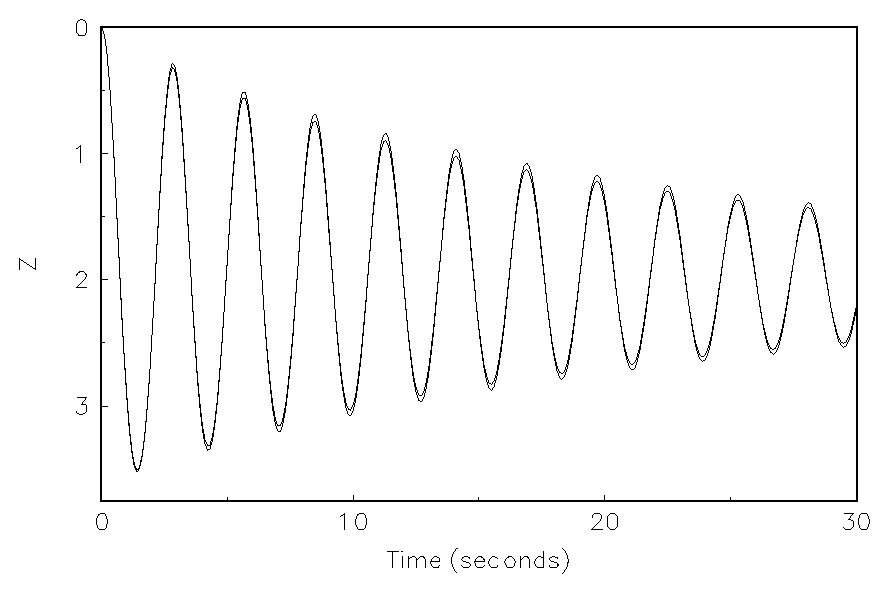
\includegraphics[width=0.75\textwidth]{fig.eps}
\caption{This figure was saved as an encapsulated Postscript file. It is also centred between the 
margins. Note that because the bounding box was rather generous some
space was removed above and below the figure. This is not a good example
of a figure; the lines should be thicker and a bigger and bolder font
used.}
\end{figure*}

\section{Equations}
Equations will be centred with a number flush against the right margin
as in
\begin{equation}\label{energy}
\rho c_p\frac{\partial T}{\partial t}=S-k\frac{\partial^2 T}{\partial x^2},
\end{equation}
and this equation would be referred to as ``equation (\ref{energy})''.

Some care should be taken in ensuring that long Mathematical
expressions are correctly split over lines. The \LaTeX\ environment
\begin{verbatim}
\begin{eqnarray}
\end{eqnarray}
\end{verbatim}
as in the equation
\begin{eqnarray}
\rho c_p\frac{\partial T}{\partial t}
&=&
S-k\frac{\partial^2 T}{\partial x^2}
\nonumber\\
& &
- k\frac{\partial^2 T}{\partial y^2}
- k\frac{\partial^2 T}{\partial z^2}
\label{11}
\end{eqnarray}
should be used. If necessary use $\times$ at the end of a line to
indicate that the multiplication is to be carried over to the next
line.

\section{Miscellaneous}
\begin{itemize}
\item Try to avoid isolated lines of text where, for example, a paragraph 
      spills over a page. Often a slight rewording resolves the problem.
\item Avoid wasted white space around figures or a last page that is
      almost empty. 
\item Use quotation marks correctly, as in ``correct'', not "incorrect".
\item Use a hyphen (-) for compound words (two-dimensional), an en-dash
      to link numbers, nouns or names (Navier--Stokes, pages 27--85), and an 
      em-dash to link clauses or sentences---like this.
\item Use a $\times$ to represent multiplication in text, not x.
\item Resist the temptation to use footnotes.
\end{itemize}

\section{Format for References}

The references are listed in alphabetical order (by first author)
and formatted as shown by the examples at the end of this paper. 
They may be referred to by the reference number alone or by the 
author(s) together with the reference number as in 
``\cite{goos} is a book, \cite{mcc} is an article in a proceedings,
\cite{rosenhead} is an edited book, and reference Cooley and Tukey \cite{cool} 
is an article in a journal.''
Multiple citations should be written as \cite{goos,rosenhead}.

Use the standard bibliography environment for references.
\begin{verbatim}
\begin{thebibliography}{1}
\end{thebibliography}{1}
\end{verbatim}

The style file \texttt{afmc.bst} (generously
contributed by Andrew Kiss of RSES, ANU) is available
for BibTeX users, who will need to put \texttt{afmc.bst} in the
BibTeX search path (e.g. \texttt{/usr/share/texmf/bibtex/bst/} on my
machine) and then put \verb/\bibliographystyle{afmc}/ in the
document preamble.
The references section is generated automatically by the command,
\verb/\bibliography{/\textsf{your\_.bib\_file\_name\_without\_the\_.bib}\verb/}/


\section{Conclusions}
You should include a brief conclusion section which summarizes the
results of your paper.

\section{Acknowledgements}
Any acknowledgements should appear immediately before the references.
This template is modified from one for the 14$^{\mbox{th}}$ AFMC in 
Adelaide 2001.
%%%%%
%%%%%%% change "1" to "11" in following line if > 10 references.
%%%%%

\begin{thebibliography}{1}
\bibitem{cool}
Cooley, J.W.~and Tukey, J.W., An Algorithm for the Machine Computation 
of Complex Fourier Series, {\em Math. Comp.}, {\bf 19}, 1965, 297--301.
\bibitem{goos}
Goosens, M., Mittlebach, F.~and Samarin, A., {\em The \LaTeX\ Companion},
Addison--Wesley, 1994.
\bibitem{mcc}
McCormick, S., Multilevel Projection Methodology, in {\em Computational
Techniques and Applications: CTAC93}, editors D. Stewart, H. Gardner and 
D. Singleton, World Scientific, 1994, 54--57.
\bibitem{rosenhead}
Rosenhead, L. editor {\em Laminar Boundary Layers} Oxford, Clarendon Press, 
1963.
\end{thebibliography}
\end{document}

% \section{Notes for MS Word users}
% The following notes are intended to assist users of MS-Word 6, so that
% their papers follow, as closely as possible, the format specified in the
% document templates.
% \begin{itemize} 
% \item The paper must be set in {\tt Times} font.
% The font sizes/type are 
% \begin{enumerate}
% \item The title is in 14.4pt (bold) 
% \item The author list is in 12pt (italic) 
% \item The address list is in 10pt (roman) 
% \item The running headers are in 9pt (roman)
% \item The figure and table captions are in 9pt (roman)
% \item The text is in 10pt (roman)
% \item The references are in 9pt (roman)
% \end{enumerate}
% \item The various dimensions of the paper are as follows 
% \begin{enumerate}
% \item The text height is 245mm
% \item The text width is 160mm
% \item The column width is 76mm
% \item The separation between the columns is 8mm
% \end{enumerate}
% \item The margins are such that
% \begin{enumerate}
% \item The title should begin 35mm from the top of the page
% \item The running headers should begin 20mm from the top of the page
% \item The bottom margin should be 26mm from bottom of the page
% \end{enumerate}
% \end{itemize}
